\section{Resultados Experimentales}

En esta sección se presentan los resultados obtenidos tras evaluar ambos modelos (LSTM y GRU) sobre el conjunto de prueba de 25,000 reseñas de IMDB. Se comparan las métricas de clasificación, los tiempos de entrenamiento y se analizan visualmente las curvas de aprendizaje, matrices de confusión y normas de gradiente.

\subsection{Métricas de Clasificación}

La Tabla~\ref{tab:comparativa_metricas} resume el rendimiento de ambos modelos en las cuatro métricas principales de clasificación binaria. El modelo GRU supera al LSTM en todas las métricas, con una diferencia de 1.34 puntos porcentuales en accuracy y 1.59 en F1-Score. La mayor diferencia se observa en recall (3.15 puntos), lo que indica que el GRU identifica mejor las reseñas positivas.

\begin{table}[H]
\centering
\caption{Comparación de métricas de clasificación entre LSTM y GRU en el conjunto de prueba (25,000 muestras).}
\label{tab:comparativa_metricas}
\begin{tabular}{lccc}
\toprule
\textbf{Métrica} & \textbf{LSTM} & \textbf{GRU} & \textbf{Diferencia} \\
\midrule
Accuracy  & 85.12\% & 86.46\% & $-1.34\%$ \\
Precision & 85.29\% & 85.34\% & $-0.05\%$ \\
Recall    & 84.88\% & 88.03\% & $-3.15\%$ \\
F1-Score  & 85.08\% & 86.67\% & $-1.59\%$ \\
\bottomrule
\end{tabular}
\end{table}

El GRU obtiene un F1-Score de 86.67\% frente al 85.08\% del LSTM. La precision es prácticamente idéntica entre ambos modelos (diferencia de 0.05\%), mientras que la diferencia principal radica en el recall: el GRU alcanza 88.03\% frente al 84.88\% del LSTM, lo que sugiere que el GRU es más sensible para detectar reseñas positivas.

\subsection{Tiempos de Entrenamiento}

Los tiempos de entrenamiento difieren significativamente entre ambas arquitecturas. El LSTM completó su entrenamiento en \textbf{71.9 segundos} con \textbf{4 épocas} antes de activar el early stopping, mientras que el GRU requirió \textbf{994.0 segundos} distribuidos en \textbf{10 épocas} completas. Esta diferencia se explica por la convergencia más rápida del LSTM en este experimento particular, que alcanzó su mejor rendimiento de validación en menos épocas.

\subsection{Curvas de Entrenamiento}

La Figura~\ref{fig:training_curves} muestra la evolución de la pérdida y la accuracy durante el entrenamiento para ambos modelos. Se observa que ambos modelos convergen de manera estable, sin oscilaciones significativas. El GRU muestra una reducción más gradual de la pérdida a lo largo de las 10 épocas, mientras que el LSTM alcanza un plateau más temprano.

\begin{figure}[H]
\centering
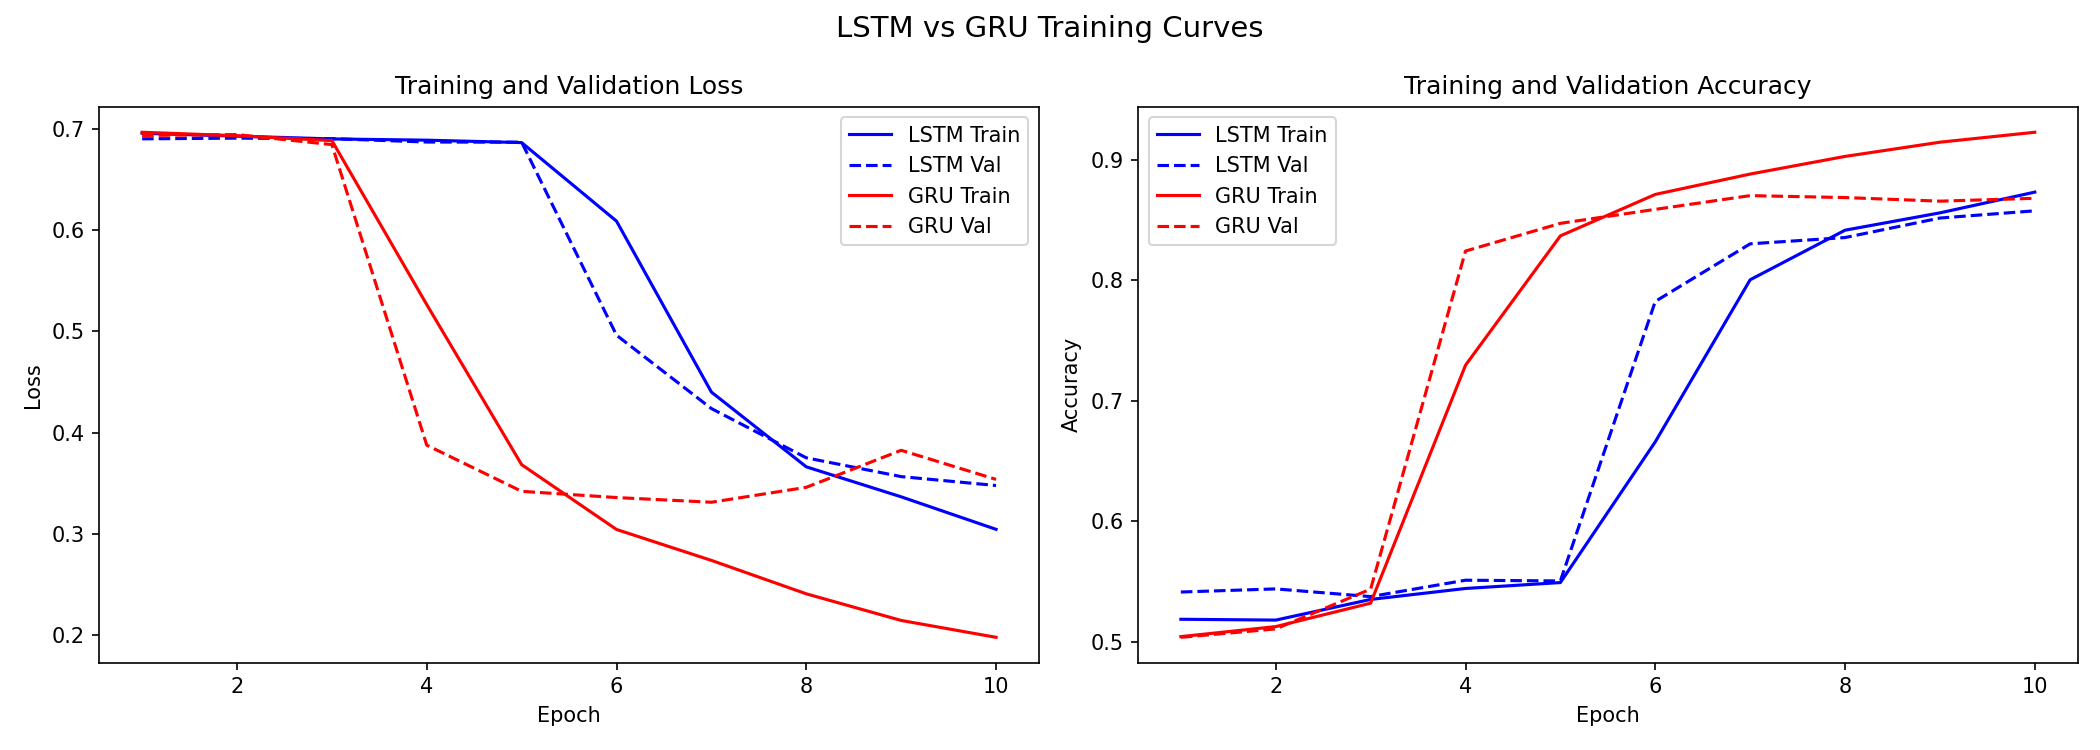
\includegraphics[width=0.9\textwidth]{img/training_curves}
\caption{Curvas de pérdida y accuracy por época para los modelos LSTM y GRU durante el entrenamiento y validación.}
\label{fig:training_curves}
\end{figure}

\subsection{Matrices de Confusión}

Las matrices de confusión presentadas en la Figura~\ref{fig:confusion_matrices} permiten visualizar la distribución de predicciones correctas e incorrectas para cada modelo. Ambos modelos muestran un comportamiento equilibrado entre las clases positiva y negativa, sin un sesgo marcado hacia ninguna de las dos.

\begin{figure}[H]
\centering
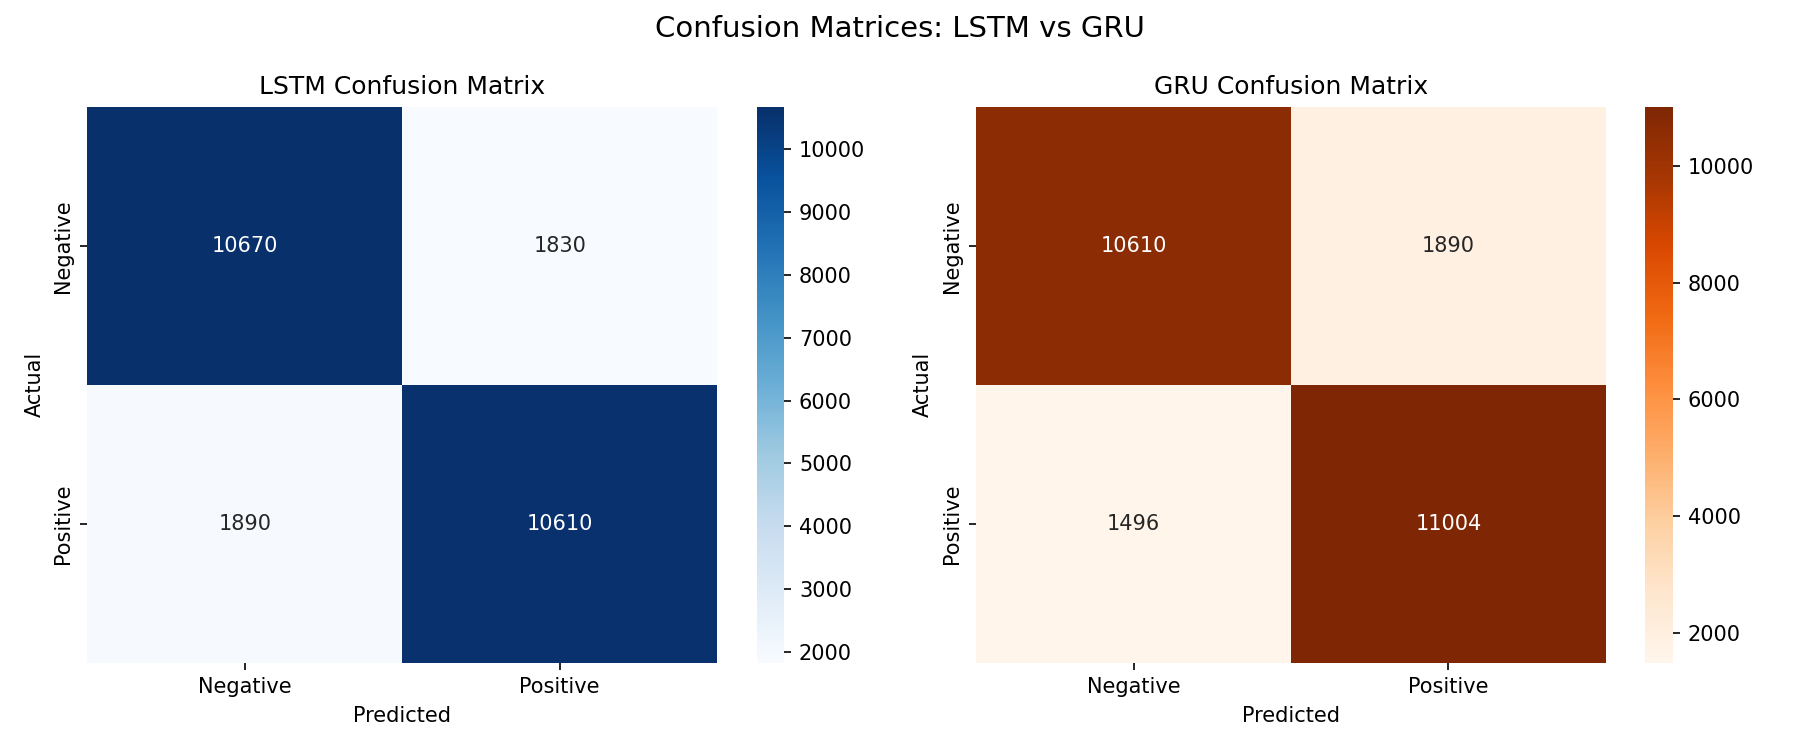
\includegraphics[width=0.9\textwidth]{img/confusion_matrices}
\caption{Matrices de confusión para los modelos LSTM (izquierda) y GRU (derecha) evaluados sobre el conjunto de prueba.}
\label{fig:confusion_matrices}
\end{figure}

\subsection{Análisis de Normas de Gradiente}

La Figura~\ref{fig:gradient_norms_resumen} presenta las normas L2 de los gradientes por capa durante los primeros 100 pasos de entrenamiento. Se observa que ambos modelos mantienen gradientes estables, sin evidencia de vanishing ni exploding gradients, lo que confirma la efectividad del gradient clipping (max\_norm=5.0) y de las compuertas internas de cada arquitectura.

\begin{figure}[H]
\centering
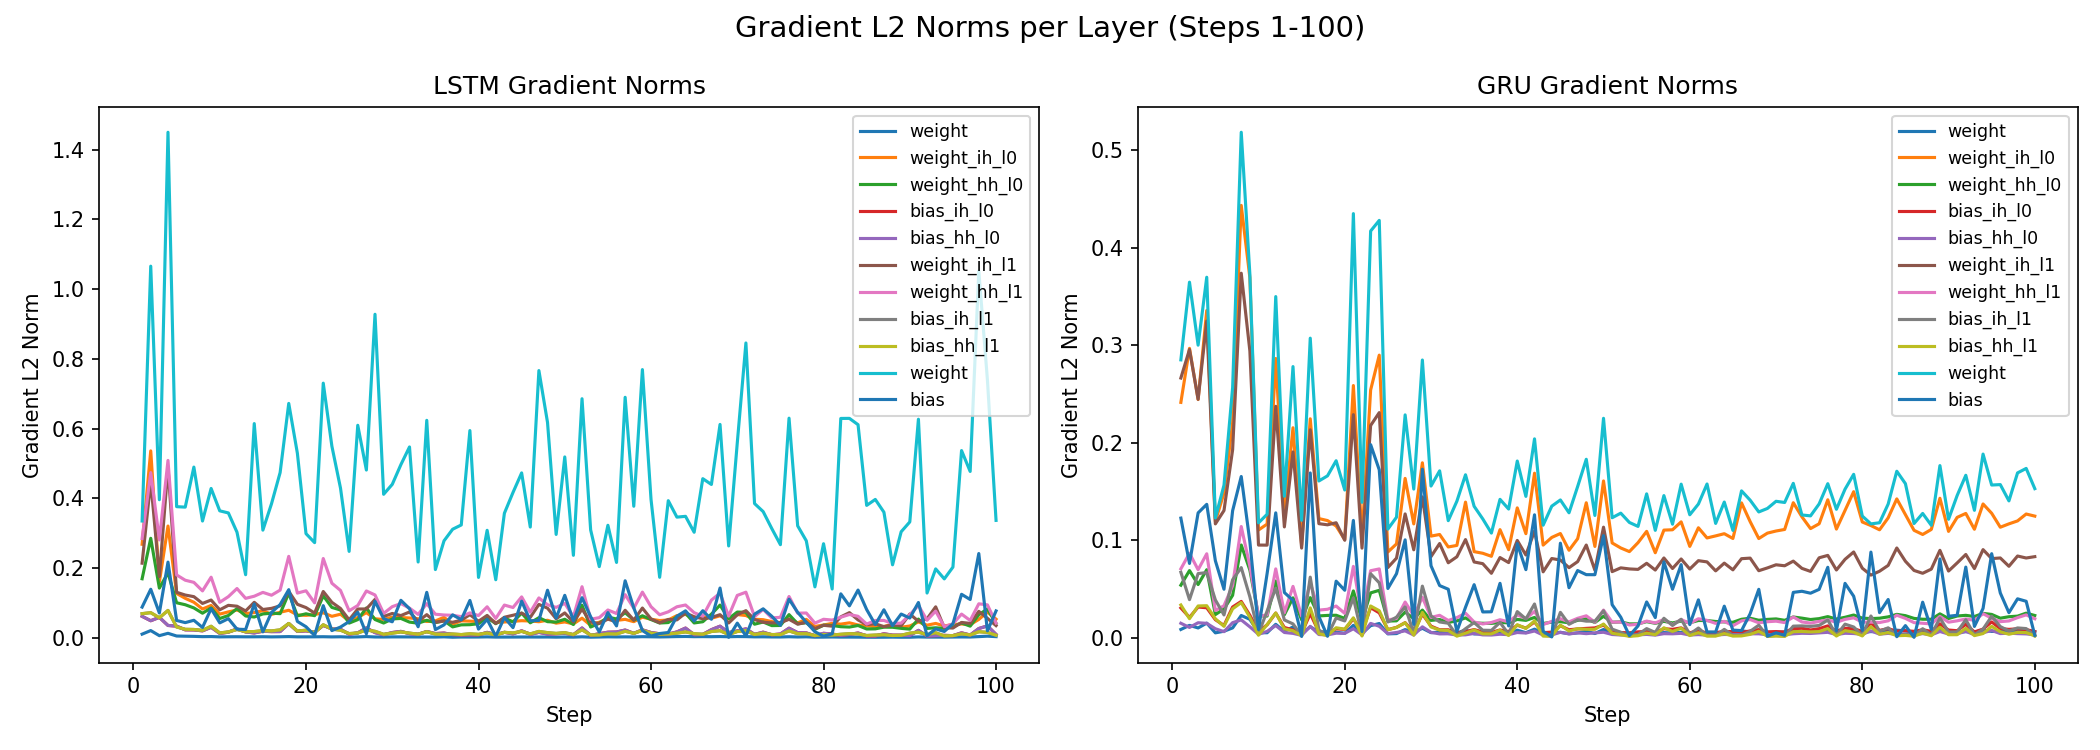
\includegraphics[width=0.9\textwidth]{img/gradient_norms}
\caption{Normas L2 de gradientes por capa durante los primeros 100 pasos de entrenamiento para LSTM y GRU.}
\label{fig:gradient_norms_resumen}
\end{figure}

\subsection{Proceso de Inferencia}

El siguiente fragmento de código muestra el proceso de evaluación implementado en \texttt{evaluate.py}. La inferencia se realiza cargando el mejor checkpoint guardado durante el entrenamiento, ejecutando el forward pass sin cálculo de gradientes y aplicando la función sigmoide con umbral de 0.5 para obtener las predicciones binarias.

% --- Inferencia: carga de checkpoint, forward sin gradientes, sigmoid > 0.5 ---
\begin{minted}{python}
def evaluate_model(
    model: nn.Module,
    test_loader: DataLoader,
    device: torch.device,
    checkpoint_path: str,
    rnn_type: str,
) -> EvaluationResults:
    # Load checkpoint weights
    state_dict = torch.load(
        checkpoint_path, map_location=device, weights_only=True
    )
    model.load_state_dict(state_dict)

    # Move model to device and set eval mode
    model = model.to(device)
    model.eval()

    all_predictions: list[int] = []
    all_labels: list[int] = []

    # Inference with no gradient computation
    with torch.no_grad():
        for inputs, labels in test_loader:
            inputs = inputs.to(device)
            labels = labels.to(device)

            # Forward pass: model outputs logits (batch_size, 1)
            logits = model(inputs).squeeze(1)

            # Apply sigmoid and threshold at 0.5
            probs = torch.sigmoid(logits)
            preds = (probs > 0.5).long()

            all_predictions.extend(preds.cpu().numpy().tolist())
            all_labels.extend(labels.cpu().numpy().tolist())
\end{minted}

Este fragmento ilustra las tres etapas clave de la inferencia: (1) carga del estado del modelo desde el checkpoint, (2) desactivación del cálculo de gradientes con \texttt{torch.no\_grad()}, y (3) aplicación de la función sigmoide seguida del umbral de decisión para convertir logits en predicciones binarias.
